\chapter{Testing}
\label{ch:testing}
\section{Introduction}
\newpage

\begin{landscape}
	\section{Requirements Testing}
	\begin{tabularx}{\hsize}{lXXXr}
		\toprule
		ID & Name & Expected Output & Evidence & Success? \\
		\midrule
		F1 & User Interaction 
		& A page should display to allow the user to interact with the bot
		& 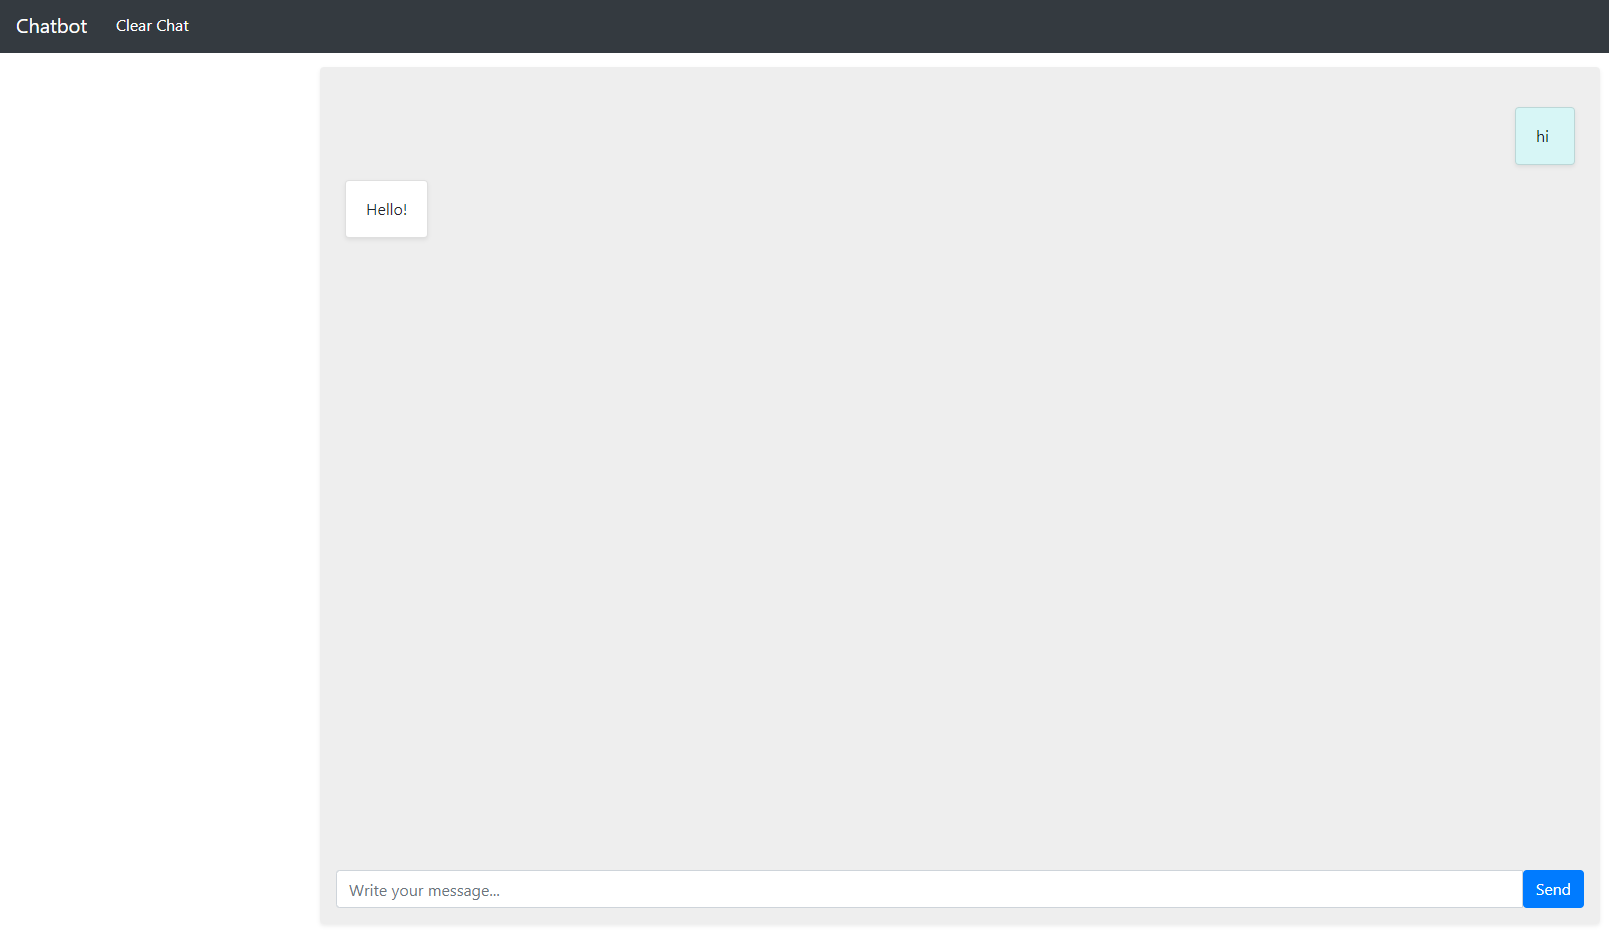
\includegraphics[width=8cm]{tests/f1} & Yes \\
		\midrule
		F2 & Browser Access
		& The user should be able to access the system via a browser
		& 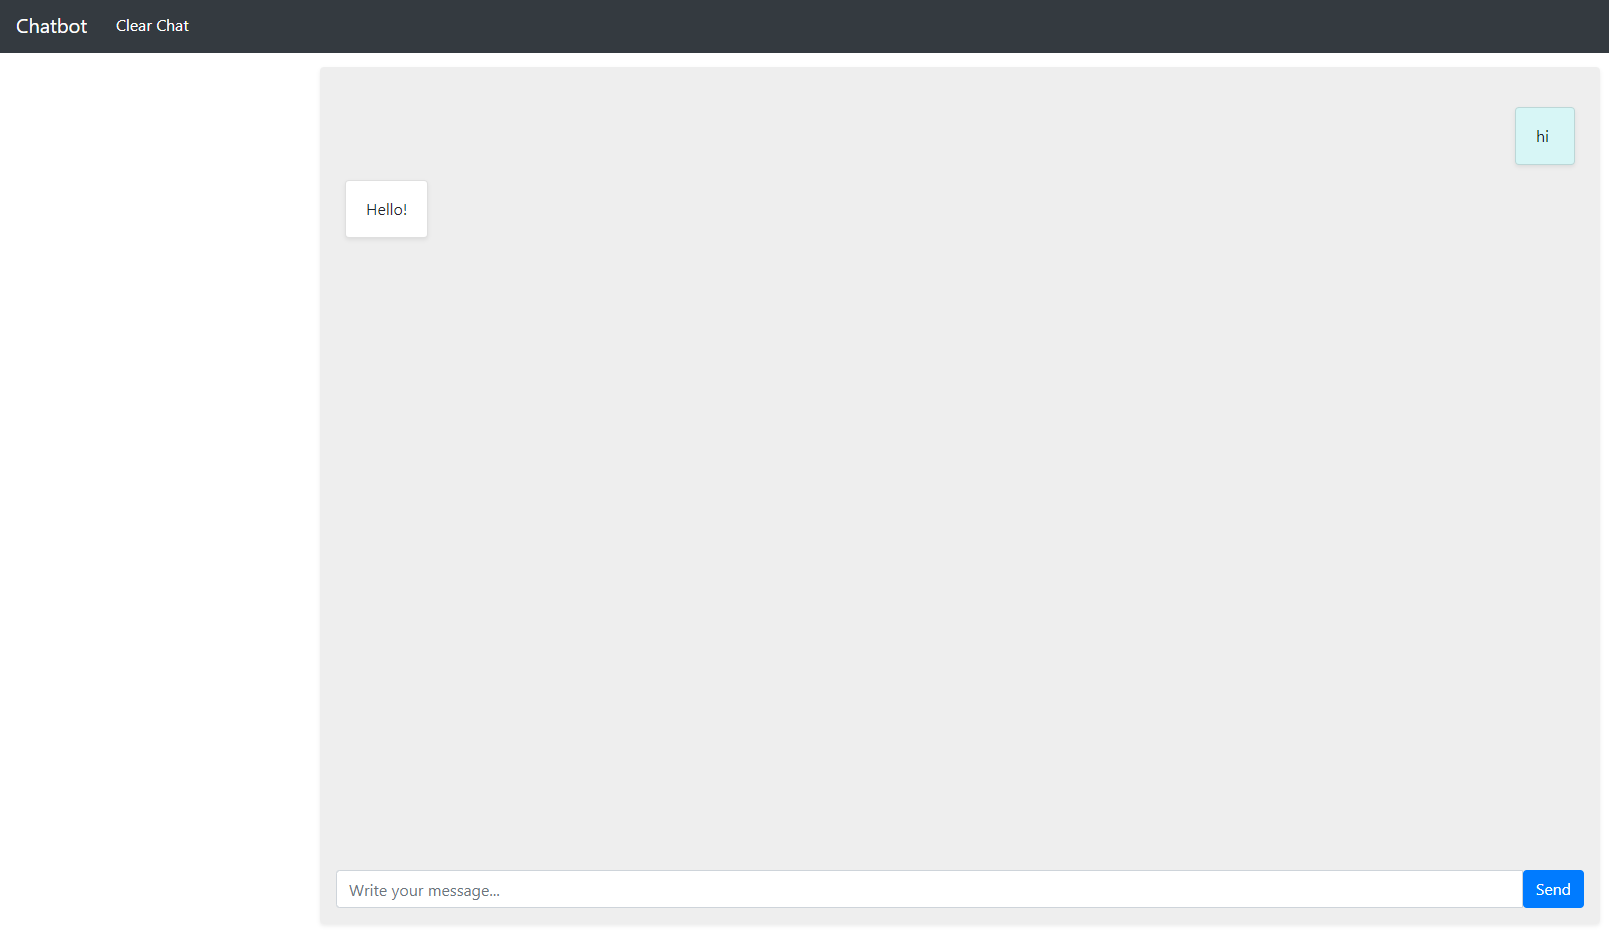
\includegraphics[width=8cm]{tests/f1} & Yes \\
		\midrule
		F3 & User Input
		& The user should be enter queries to the bot using a textbox input
		& 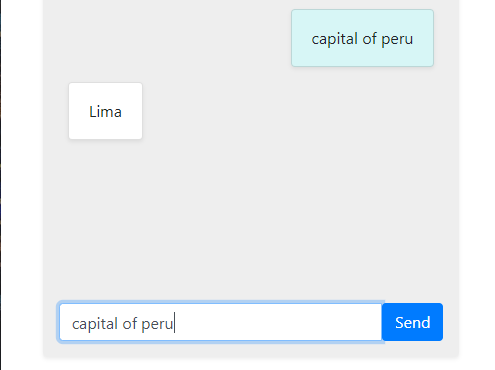
\includegraphics[width=8cm]{tests/f3} & Yes \\
		\bottomrule
		F4 & Responses on Page
		& The should see the chatbot response on the web page
		& 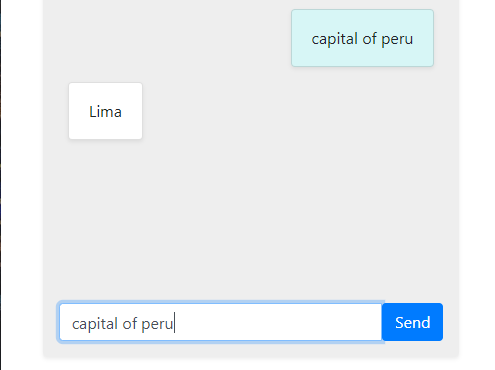
\includegraphics[width=8cm]{tests/f3} & Yes \\
		\bottomrule
		F5 & Conversation History
		& The should see the whole conversation with the bot on the page
		& 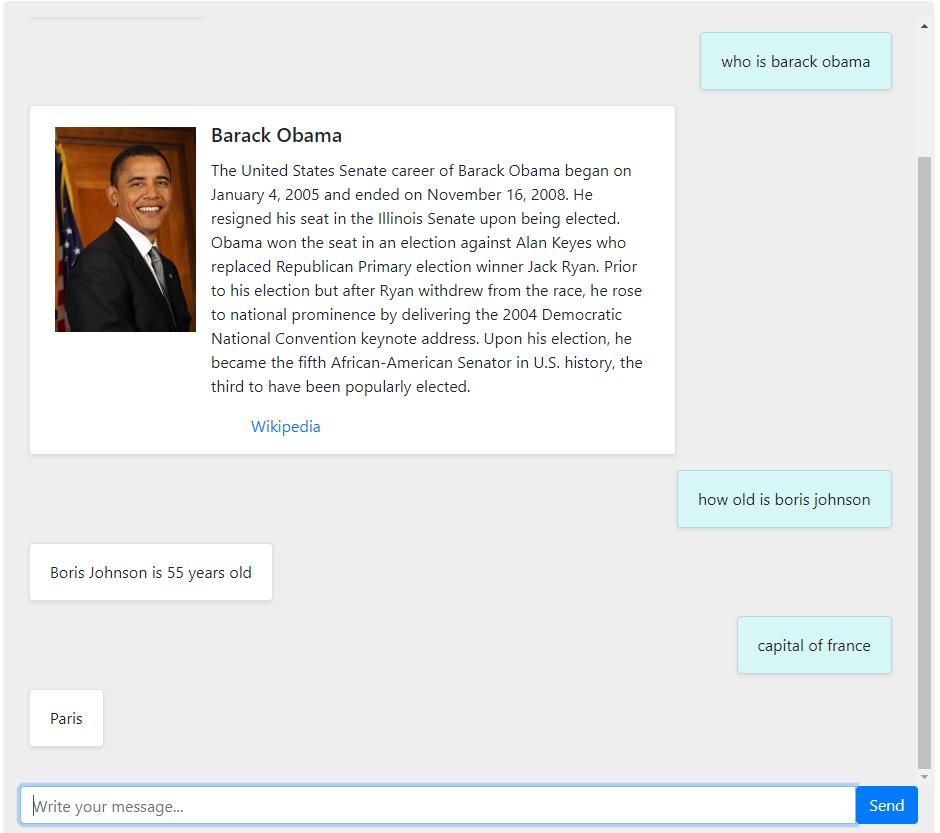
\includegraphics[width=8cm]{tests/f5} & Yes \\
		\bottomrule
		F6 & Person Description Query
		& The user should be able to ask a query about who a person is\newline - 'WHO IS *' and receive a description of that person
		& 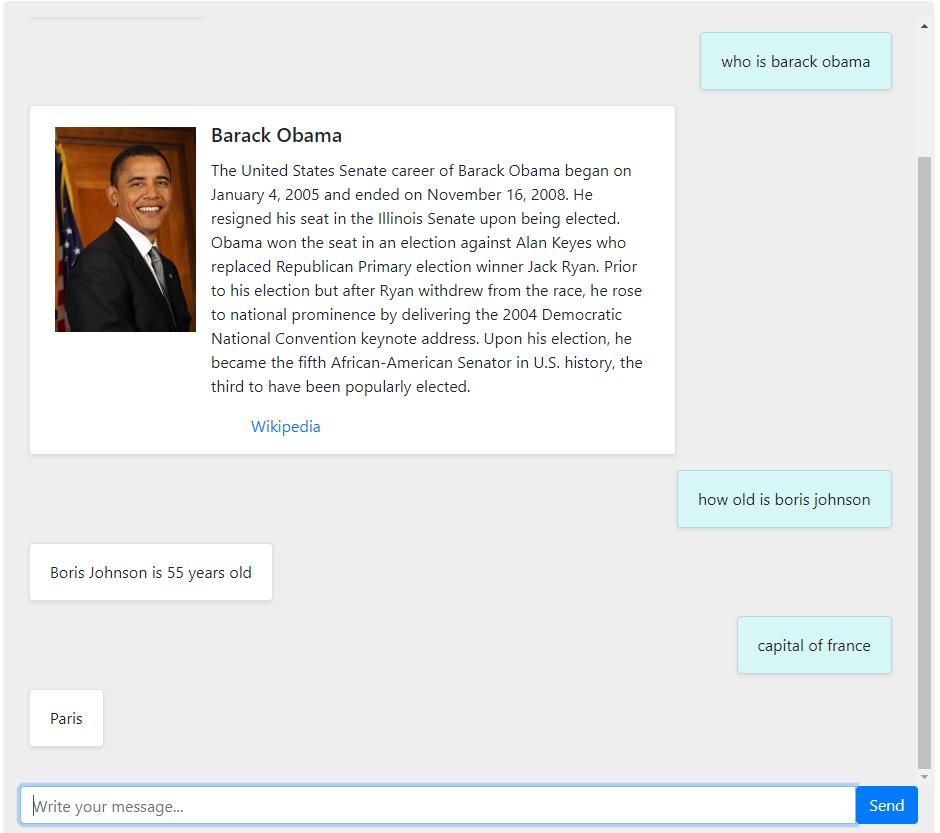
\includegraphics[width=8cm]{tests/f5} & Yes \\
		\bottomrule
		F7 & Person Birthdate Query
		& The user should be able to ask a query about when a person was born\newline - 'WHEN WAS * BORN' and see their birth date
		& 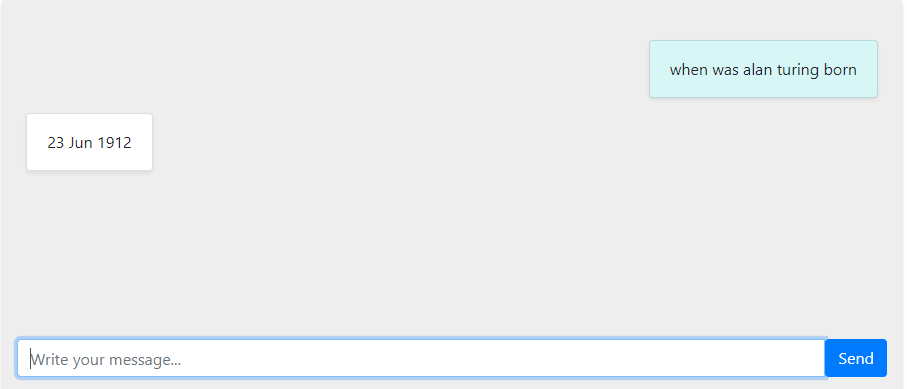
\includegraphics[width=8cm]{tests/f7} & Yes \\
		\bottomrule
		F8 & Person Age Query
		& The user should be able to ask a query about a person's age\newline - 'HOW OLD IS *' and see their age
		& 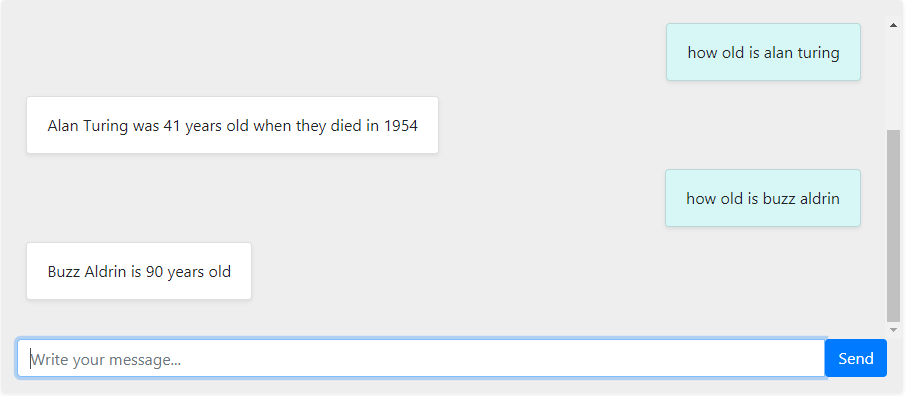
\includegraphics[width=8cm]{tests/f8} & Yes \\
		\bottomrule
		F9 & Person Birthplace Query
		& The user should be able to ask a query about where a person was born\newline - 'WHEN WAS * BORN' and see their birthplace
		& 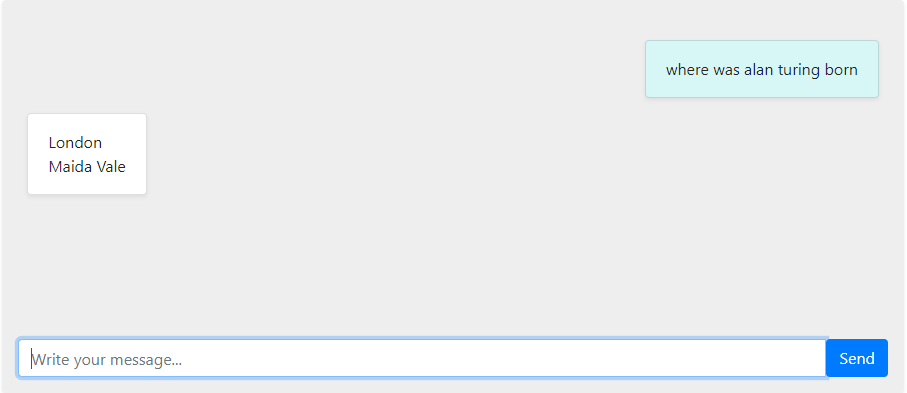
\includegraphics[width=8cm]{tests/f9} & Yes \\
		\bottomrule
		F10 & Person Death Date query
		& The user should be able to ask a query about when a person died\newline - 'WHEN DID * DIE' and see their death date
		& 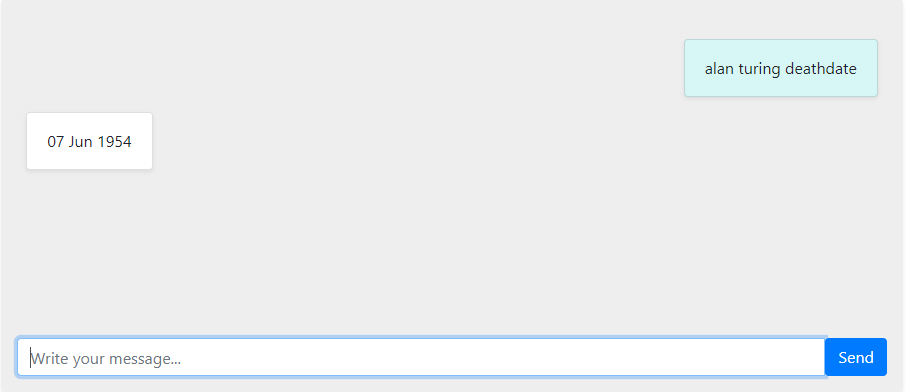
\includegraphics[width=8cm]{tests/f10} & Yes \\
		\bottomrule
		F11 & Person Known For Query
		& The user should be able to ask a query about what a person is known for\newline - 'WHAT IS * KNOWN FOR' and see what they are known for
		& 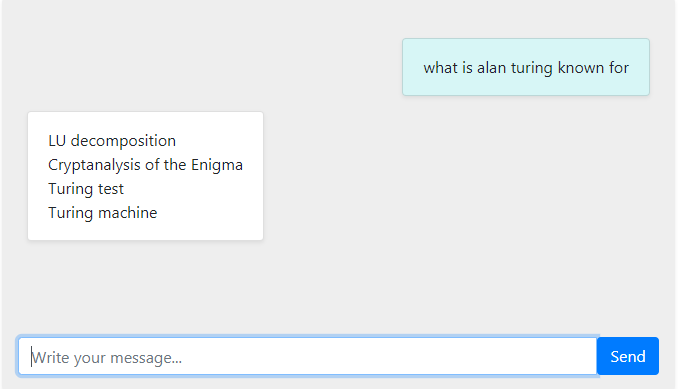
\includegraphics[width=8cm]{tests/f11} & Yes \\
		\bottomrule
		F12 & Person Photo Query
		& The user should be able to ask for a photo of a person\newline - 'WHAT DOES * LOOK LIKE' and see a photo of the person
		& 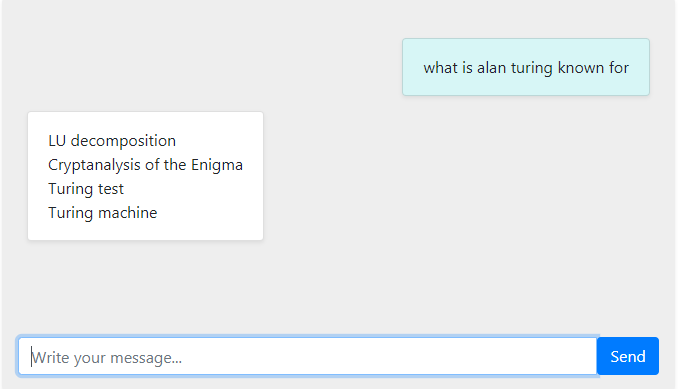
\includegraphics[width=8cm]{tests/f11} & Yes \\
		\bottomrule
		F13 & Person Wikipedia Link Query
		& The user should be able to ask for the link to a person's Wikipedia page\newline - '* WIKIPEDIA PAGE' and receive a link to their page
		& 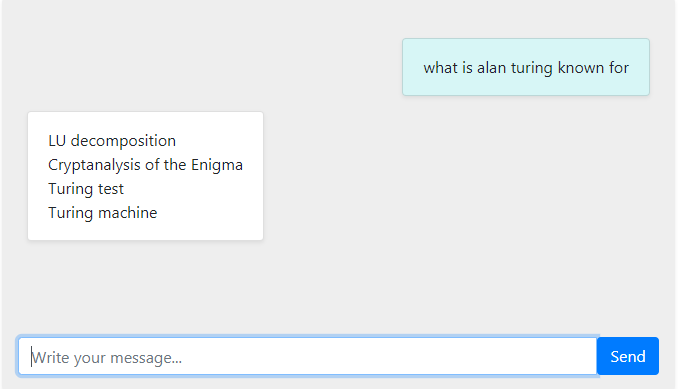
\includegraphics[width=8cm]{tests/f11} & Yes \\
		\bottomrule
		F14 & Country Description Query
		& The user should be able to ask about a country\newline - '[COUNTRY]' and see a description of that country
		& 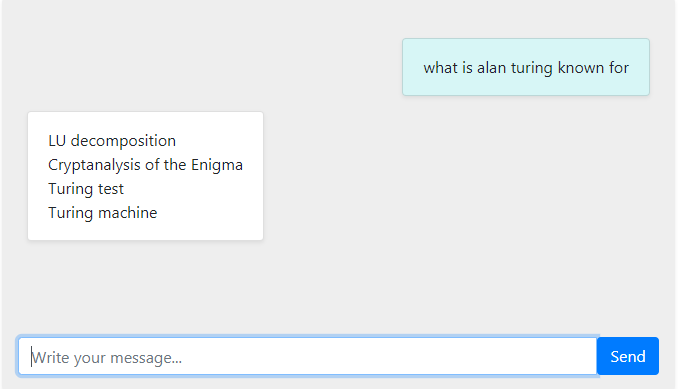
\includegraphics[width=8cm]{tests/f11} & Yes \\
		\bottomrule
		F15 & Country Population Query
		& The user should be able to ask about a country\newline - '[COUNTRY] POPULATION' and see the population of that country
		& 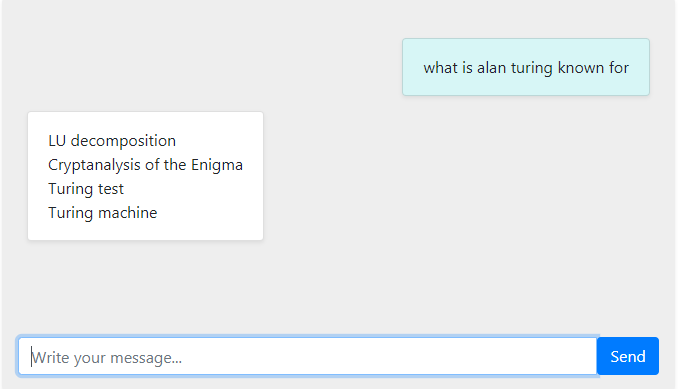
\includegraphics[width=8cm]{tests/f11} & Yes \\
		\bottomrule
		F16 & Country Capital Query
		& The user should be able to ask for the capital of a country\newline - 'CAPITAL OF [COUNTRY]' and see the capital of that country
		& 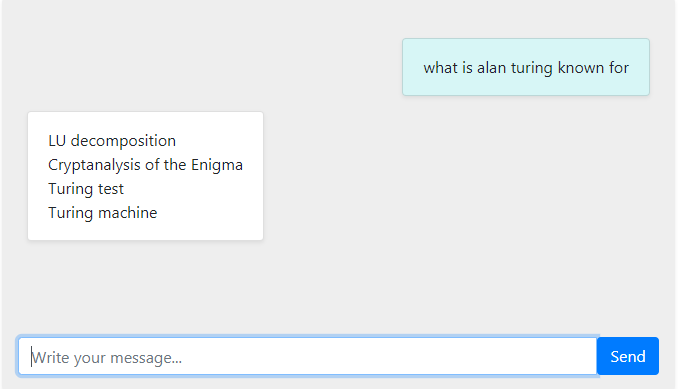
\includegraphics[width=8cm]{tests/f11} & Yes \\
		\bottomrule
		F17 & Person List Query
		& The user should be able to ask for lists of people\newline - 'LIST OF ACTORS' - and see a list of actors 
		& 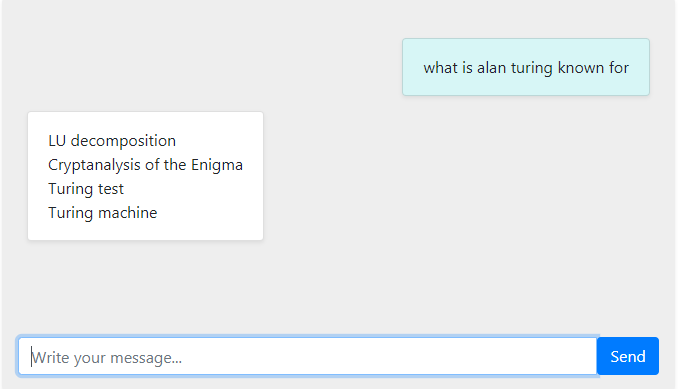
\includegraphics[width=8cm]{tests/f11} & Yes \\
		\bottomrule
		F18 & Person AND Query
		& The user should be able to combine queries\newline - 'LIST OF ACTORS BORN IN 1990 AND BORN IN LONDON'\newline and see a list matching that conditional query
		& 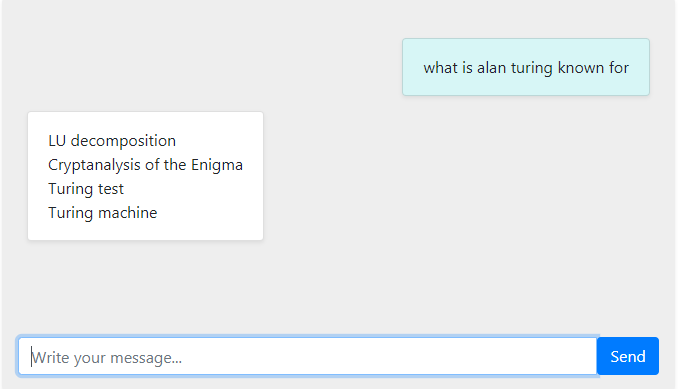
\includegraphics[width=8cm]{tests/f11} & Yes \\
		\bottomrule
		F19 & Context-aware Conversation
		& The user should be able to continue from previous queries using pronouns\newline e.g. 'WHEN WAS HE BORN' and the chatbot should maintain the context of the query
		& 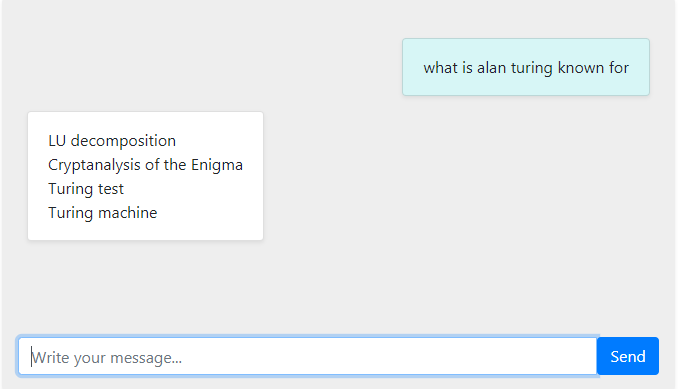
\includegraphics[width=8cm]{tests/f11} & Yes \\
		\bottomrule
		F20 & Chatbot Greeting
		& The chatbot should be able to greet the user
		& 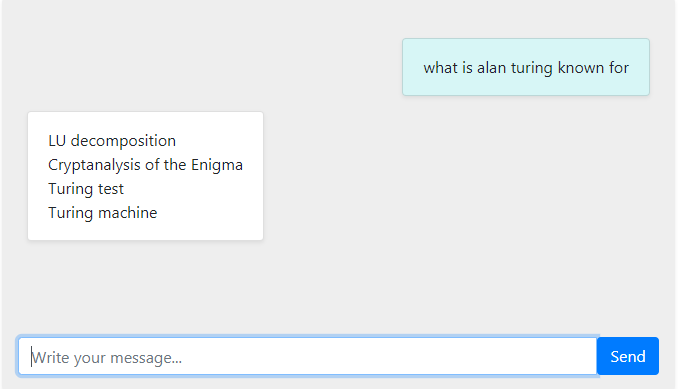
\includegraphics[width=8cm]{tests/f11} & Yes \\
		\bottomrule
		F21 & Chatbot Examples
		& The chatbot should display a list of example queries\newline when asked 'EXAMPLES' or 'WHAT CAN YOU DO'
		& 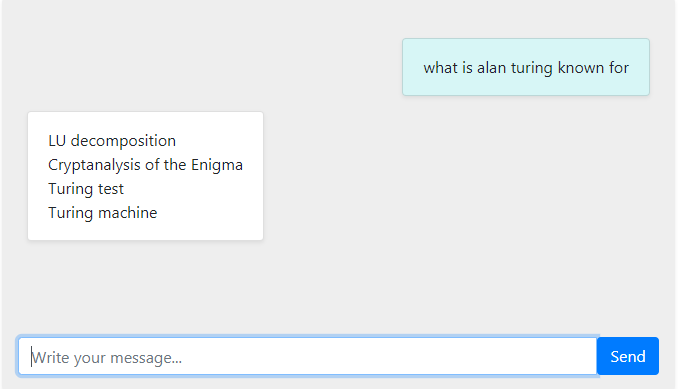
\includegraphics[width=8cm]{tests/f11} & Yes \\
		\bottomrule
		F22 & Chatbot Help
		& The user should be able to receive help from the chatbot\newline on how to use it when asked 'HELP'
		& 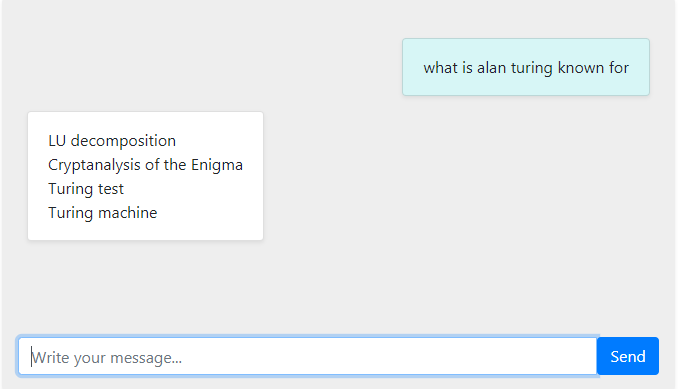
\includegraphics[width=8cm]{tests/f11} & Yes \\
		\bottomrule
		P1 & Web page loads in 5 seconds
		& 
		& 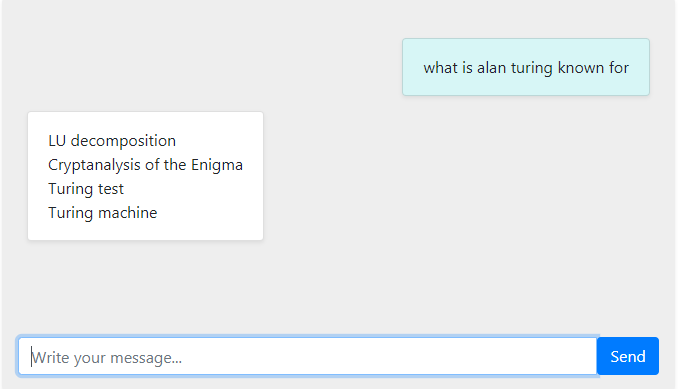
\includegraphics[width=8cm]{tests/f11} & Yes \\
		\bottomrule
		P2 & Chatbot responds in 5 seconds
		& 
		& 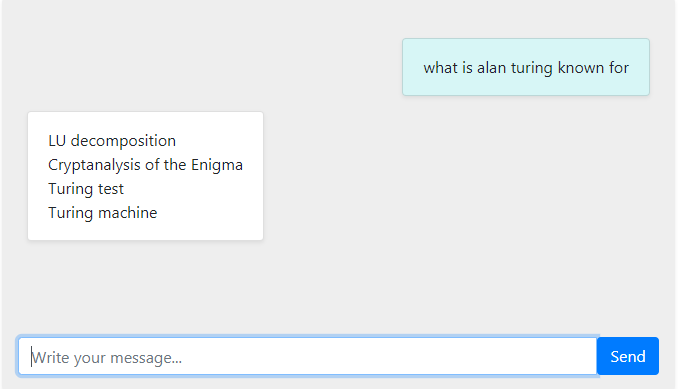
\includegraphics[width=8cm]{tests/f11} & Yes \\
		\bottomrule
		P3 & Application functions without failure
		& 
		& 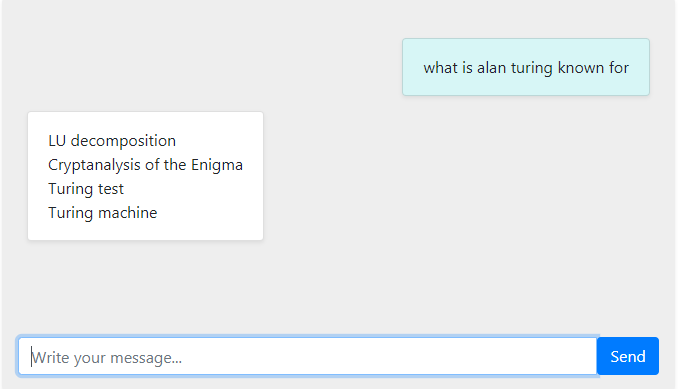
\includegraphics[width=8cm]{tests/f11} & Yes \\
		\bottomrule
		P4 & Any errors are logs and the user is informed
		& 
		& 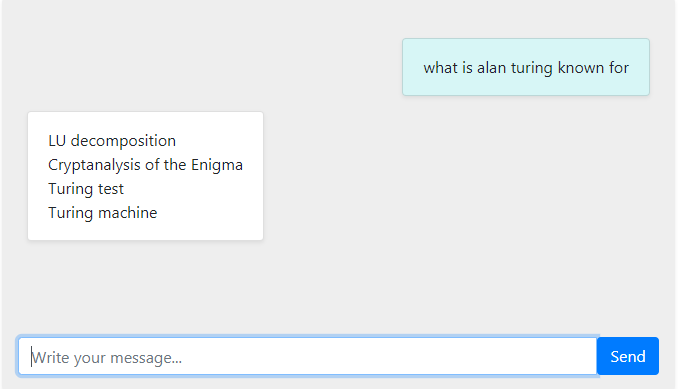
\includegraphics[width=8cm]{tests/f11} & Yes \\
		\bottomrule
		%\caption{Requirements testing and evidence}
		%\label{tab:testreq}
	\end{tabularx}
\end{landscape}


\newpage
\section{Unit Testing}
\section{User Acceptance Testing}
\section{Conclusion}